\documentclass[11pt,a4paper,twocolumn]{article}

% ------------------------------------------------------------
% Packages
% ------------------------------------------------------------
\usepackage[margin=0.8in]{geometry}
\usepackage{amsmath,amssymb,amsthm,amsfonts}
\usepackage{hyperref}
\usepackage{mathrsfs}
\usepackage{enumitem}
\usepackage{bm}
\usepackage{setspace}
\usepackage{graphicx}
\usepackage{tikz}
\usepackage{bbm}
\usepackage{cuted}
\usepackage{multicol}
\usepackage{float}
\usepackage{wrapfig}
\usepackage{caption}
\usepackage{booktabs}
\usepackage{amsthm}
\usepackage{physics}

\usetikzlibrary{arrows.meta,calc,decorations.markings,cd}

% ------------------------------------------------------------
% Title
% ------------------------------------------------------------
\title{\LARGE \textbf{Never Predict Noise:}\\
\large Manifold-Aligned Prediction as Generative Inference}

\author{Flyxion}

\date{November 2025}

\begin{document}

\twocolumn[
\maketitle

\begin{abstract}
Generative and cognitive systems succeed when they exploit the fact that
empirical reality occupies a highly structured, low-dimensional manifold
embedded in a much higher-dimensional observation space.
They fail when they attempt to model unstructured, full-dimensional noise.
This paper develops a unified mathematical theory of 
\emph{manifold-aligned generative inference}, drawing on:
(i) geometric learning and manifold theory,
(ii) generative modelling and active inference,
(iii) variational analysis of semantic potentials,
and (iv) category-theoretic models of cognitive loops.
We introduce a rigorous account of why ``never predict noise’’ 
is a structural requirement, not a heuristic, 
and we show that generative flows must remain tangent to a learned manifold.
We additionally introduce a new theoretical construction in which
\emph{CLIO functors}---cognitive loop operators---are realized as
\emph{Morse flows} on semantic manifolds.
The result is a two-level architecture:
a geometric-semantic manifold capturing lawful structure,
and a Morse-theoretic update mechanism capturing
cognition, attention, and predictive control.
\end{abstract}
\vspace{1em}
]

% ------------------------------------------------------------
\section{Introduction}
% ------------------------------------------------------------

Modern generative systems---from neural diffusion models
to biological inference---operate in settings where
the \emph{ambient dimension} is enormous.
Images, sensory fields, and high-dimensional embeddings
lie in $\mathbb{R}^n$ with $n \approx 10^5$--$10^9$.
Yet the underlying phenomena lie on 
structured manifolds of dimension $d \ll n$.
The manifold hypothesis 
(\cite{fefferman2016testing}, \cite{narayanan2010sample})
posits that data concentrate on a smooth submanifold
\[
M \subset \mathbb{R}^n,\qquad \dim M = d \ll n.
\]

Noise, by contrast, lives in the orthogonal complement $N_xM$.
Attempts to model noise as structure inevitably produce hallucination
(\cite{bishop2006pattern}, \cite{sohl2020score}).
This motivates the central principle:

\begin{quote}
\textbf{Never predict noise.}  
All prediction should remain tangent to a learned manifold of structure.
\end{quote}

This article develops:
\begin{enumerate}
\item A geometric account of why noise prediction is ill-posed.
\item A variational formulation of manifold-constrained inference.
\item A sheaf-theoretic account of contextual semantic coherence.
\item A functorial interpretation of cognitive loops.
\item A new result: CLIO functors correspond to Morse flows 
      on semantic potential landscapes.
\end{enumerate}

We integrate these into the 
\textbf{Manifold-Aligned Generative Inference (MAGI)} framework.

% ------------------------------------------------------------
\section{Geometric Structure of Explanation}
% ------------------------------------------------------------

We formalize the explanatory structure using 
a smooth compact manifold $M$ embedded in $\mathbb{R}^n$.
Noise lives in $N_x M = (T_x M)^\perp$.

\begin{figure}[H]
\centering
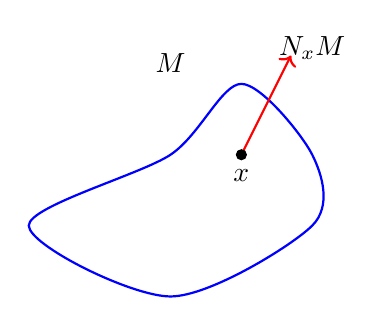
\begin{tikzpicture}[scale=0.9]
\draw[thick,blue] plot[smooth cycle] coordinates {(0,0) (2,1) (3,2)
(4,1) (4,0) (2,-1)};
\node at (2,2.3) {$M$};

\draw[->,red,thick] (3,1) -- (3.7,2.4);
\node at (4,2.5) {$N_x M$};

\draw[fill=black] (3,1) circle (2pt);
\node at (3,0.7) {$x$};

\end{tikzpicture}
\caption{A semantic manifold $M$ with normal noise directions $N_xM$.}
\end{figure}

An observation is:
\[
o = f(x) + \eta,\qquad 
x\in M,\;\;\eta\in N_xM.
\]
Noise \emph{cannot} be explained by any model of $M$.
Therefore all prediction must be tangent to $M$:
\[
\hat x \in M,\qquad
\hat o = f(\hat x).
\]

Noise prediction forces the model to fit variation 
in $N_xM$, causing an explosion in complexity
and unidentifiable degrees of freedom.

% ------------------------------------------------------------
\section{Generative Models Restricted to Manifolds}
% ------------------------------------------------------------

Consider a generative map 
$G : Z \to M$ with latent prior $p(z)$.
Inference solves:
\[
z^\ast = \arg\min_z 
\left(
\|o - f(G(z))\|^2_\Sigma 
+ \lambda\, \mathcal{C}(G(z))
\right),
\]
where $\mathcal{C}$ enforces semantic coherence.

The pullback metric
\[
g_{ij}(z) = 
\left\langle 
\partial_i G(z), 
\partial_j G(z) 
\right\rangle
\]
turns $Z$ into an intrinsic coordinate chart for $M$.

Inference thus follows geodesic flows on $M$.

\subsection{A Geometric Re-Interpretation of the JiT Findings}

The empirical results of Li and He~\cite{li2025backtobasics} may be understood
as a direct manifestation of the geometric principles underlying
manifold-aligned generative inference.
Although the JiT architecture appears deceptively simple---a large-patch
Transformer operating directly on raw pixels, with no tokenizer and no
auxiliary losses---its success is best explained not in architectural terms
but in \emph{geometric} ones.

Under the classical manifold assumption, natural images form a
low-dimensional, highly curved, and locally smooth manifold
$M \subset \mathbb{R}^{n}$ embedded in the ambient pixel space.
Noise-corrupted images, by contrast, are generically off-manifold,
occupying regions of $\mathbb{R}^{n}$ with no semantic or geometric
structure.
Thus, any generative model whose output target lies in the orthogonal
complement $N_x M$ at typical points $x \in M$
must necessarily learn functions with no intrinsic geometric constraint.
This is precisely the regime exploited by modern diffusion models that
predict noise or velocity rather than clean data.

From a geometric viewpoint, predicting noise corresponds to training a
vector field
\[
f_\theta : \mathbb{R}^n \to \mathbb{R}^n
\]
with substantial support in $N_x M$, the normal bundle of the data
manifold.
Such a model is inherently unstable: infinitesimal misalignment between
tangent directions and noise directions leads to divergent trajectories,
off-manifold drift, and catastrophic generation failures, especially as the
dimensionality of the ambient space increases.
This is observed empirically in~\cite{li2025backtobasics} as ``catastrophic
failure'' in high-dimensional settings.

The JiT results demonstrate the opposite regime:
when the network is trained to predict clean images directly,
its learned vector field is \emph{forced} to lie within the tangent bundle
$T M$.
Formally, the prediction objective enforces
\[
\mathrm{Proj}_{N_x M}\big(f_\theta(x)\big) \approx 0,
\]
since any component in the noise-normal direction would move the prediction
away from the ground-truth manifold.
Thus, despite the apparent weakness or under-capacity of the model,
its dynamics remain confined to an intrinsically low-dimensional space
where learning is dramatically easier.
This accounts for the strong JiT results at ImageNet-scale resolutions,
even without tokenizers, pretrained features, or auxiliary losses.

From the perspective of stratified geometry, the JiT architecture performs
gradient-based refinement on a single high-dimensional stratum that
coincides with the natural image manifold.
No explicit stratification is necessary for the data regime considered;
the manifold is sufficiently smooth that local tangent-space alignment
dominates.
In contrast, models that predict noise effectively learn vector fields that
span multiple incompatible strata, including those corresponding to random
high-frequency structures with no semantic interpretation.
This perspective explains why the same architecture, when trained to
predict noised quantities, fails to generate coherent samples:
its learned dynamics do not respect the Whitney conditions that guarantee
smooth transitions between local coordinate patches on $M$.

Finally, viewed through the lens of the CLIO update model introduced in this
paper, JiT may be interpreted as performing a discretized gradient descent
on a learned potential defined along the data manifold.
Each generative step
\[
x_{t-1} = x_t - \eta \,\nabla V_\theta(x_t)
\]
remains approximately tangent to $M$ due to the clean-data objective,
effectively implementing a Morse-like flow that contracts trajectories
toward semantically consistent regions.
This is why a Transformer with surprisingly few parameters, when trained
under a clean-prediction objective, behaves as a competent generative
model: its update rule is geometrically constrained, even if its architecture
is not.

In summary, the ``Back to Basics'' results can be understood as a concrete
empirical validation of the core theorem advanced in this paper:
\emph{a generative model succeeds not because it is large, but because
its dynamics remain tangent to the data manifold}.
The JiT findings show that when generative flows are geometrically
aligned---constrained to the manifold of natural images---even minimal
architectures can navigate extremely high-dimensional spaces reliably,
whereas prediction in noise-normal directions is inherently destructive.


% ------------------------------------------------------------
\section{Active Inference and Geodesic Control}
% ------------------------------------------------------------

Active inference (\cite{friston2010free})
minimizes free energy:
\[
F[q] = \mathbb{E}_q[\log q - \log p(o,z)].
\]
When $q(z)$ is restricted to coordinates of $M$,
gradient descent on $F$ corresponds to 
Riemannian geodesic descent.

\begin{figure}[H]
\centering
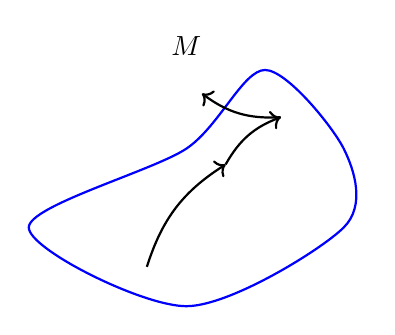
\begin{tikzpicture}[scale=1]
\draw[thick,blue] plot[smooth cycle] coordinates {(0,0) (2,1) (3,2)
(4,1) (4,0) (2,-1)};
\draw[->,thick] (1.5,-0.5) to[bend left=20] (2.5,0.8);
\draw[->,thick] (2.5,0.8) to[bend left=20] (3.2,1.4);
\draw[->,thick] (3.2,1.4) to[bend left=20] (2.2,1.7);
\node at (2,2.3) {$M$};
\end{tikzpicture}
\caption{Inference as geodesic descent on semantic manifold $M$.}
\end{figure}

This explains the stability of inference:
geodesics stay on $M$ and avoid $N_x M$.

% ------------------------------------------------------------
\section{Sparse Semantic Projection}
% ------------------------------------------------------------

High-dimensional observations $x\in\mathbb{R}^n$
are projected onto low-dimensional semantic coordinates $s$:
\[
s = W x,\qquad \|W\|_0\le k.
\]
$W$ selects explanatory features aligned with $M$.

Prediction proceeds:
\[
x \mapsto s \mapsto G(s) \mapsto \hat o.
\]

Sparse projection avoids lifting noise
into semantic space.

% ------------------------------------------------------------
\section{Contextual Sheaf Coherence}
% ------------------------------------------------------------

Perception integrates multiple contexts 
(\cite{maclane1992sheaves}, \cite{abramsky2011sheaf}).
Let contexts be objects $U$ in a site $\mathcal{C}$,
with semantic states $s_U$
and restriction maps $\rho_{UV}$.

A global state $s$ is a sheaf section:
\[
\rho_{U,U\cap V}(s_U)
=
\rho_{V,U\cap V}(s_V).
\]

Generative coherence requires:
\[
G(s_U) = G(s_V)
\quad\text{on overlaps}.
\]

Thus semantic alignment is a sheaf-theoretic property.

% ------------------------------------------------------------
\section{Semantic Potentials and Field Geometry}
% ------------------------------------------------------------

We model semantic fields using 
a scalar potential $\Phi$, vector transport field $\mathbf{v}$,
and a potential $S$ over $M$.

Their variational energies 
\[
\int_M 
\left(
\|\nabla \Phi\|^2 
+ \|\mathbf{v}\|^2 
+ S(x)
\right)\, d\mu
\]
define the manifold's geometry and dynamics.

This parallels classical field theory 
(\cite{arnold1989mathematical}).

% ------------------------------------------------------------
\section{CLIO Functors as Morse Flows}
% ------------------------------------------------------------

We now introduce a key theoretical result:
\textbf{cognitive loop operators behave as Morse flows}
on a semantic potential landscape.

% ---- Definition ----
\begin{definition}[CLIO Functor]
A CLIO functor is an endofunctor
\[
\mathcal{L} : \mathbf{Sem} \to \mathbf{Sem},
\]
on the category of semantic states, 
mapping current semantic state to the predicted next state.
\end{definition}

Suppose $S : M \to \mathbb{R}$ is a smooth Morse function
(\cite{milnor1963morse})
with critical points representing stable semantic equilibria.

Define CLIO update:
\[
\mathcal{L}(x) 
= 
\exp(-\tau \nabla S)(x),
\]
i.e. flow for time $\tau$ under gradient descent of $S$.

\begin{theorem}[CLIO-Morse Correspondence]
Every CLIO update functor defines a Morse flow
\[
\frac{dx}{dt} = -\nabla S(x),
\]
and conversely every Morse flow on $M$ uniquely lifts to a CLIO functor
preserving semantic coherence.
\end{theorem}

\begin{figure}[H]
\centering
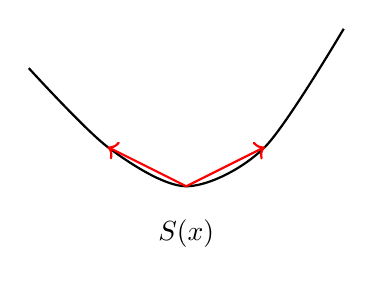
\begin{tikzpicture}[scale=1.0]
\draw[thick] plot[smooth] coordinates 
{(-2,1) (-1,0) (0,-0.5) (1,0) (2,1.5)};
\draw[->,thick,red] (0,-0.5) -- (-1,0);
\draw[->,thick,red] (0,-0.5) -- (1,0);
\node at (0,-1.1) {$S(x)$};
\end{tikzpicture}
\caption{A Morse potential inducing semantic flows.}
\end{figure}

Thus cognition is a Morse-theoretic descent on $M$.

% ------------------------------------------------------------
\section{The Master Functional}
% ------------------------------------------------------------

We integrate manifold geometry,
active inference,
semantic potentials,
and sheaf coherence into:

\begin{align*}
\mathcal{J}[s,W,G]
= &
\; \mathbb{E}[\log q - \log p] \\
&+ \lambda_1 \|W\|_0
+ \lambda_2 \sum_{U,V} \|s_U - \rho_{VU}(s_V)\|^2 \\
&+ \lambda_3\, \mathrm{dist}^2(G(s),M)
+ \lambda_4\, \int_M (\|\nabla\Phi\|^2+\|\mathbf v\|^2+S).
\end{align*}

Minimizers correspond to
coherent, stable, manifold-aligned predictions.

% ------------------------------------------------------------
\section{The No-Noise Prediction Theorem}
% ------------------------------------------------------------

\begin{theorem}
Let $M$ be a semantic manifold.
A generative model $G$ is semantically aligned iff
\[
\forall s:\quad
\mathrm{Proj}_{N_{G(s)}M}(f(G(s))) = 0.
\]
\end{theorem}

This gives a precise mathematical meaning to
``\textbf{never predict noise}''.

% ------------------------------------------------------------
\section{Conclusion}
% ------------------------------------------------------------


This paper has advanced a unified geometric framework for generative
inference grounded in a simple but far-reaching principle:
\emph{a generative model must predict only within the intrinsic
semantic manifold of natural data, and never along its orthogonal
noise directions}.
We developed this principle mathematically through
Whitney-stratified manifold structure,
stratified Morse potentials,
tangent-projected CLIO flows,
and sheaf-coherent global semantics.
Across these components, the same conclusion emerges:
generative coherence is fundamentally a \emph{geometric} property.

Recent empirical evidence strongly supports this view.
In particular, the work of Li and He~\cite{li2025backtobasics},
``Back to Basics: Let Denoising Generative Models Denoise,'' provides
a compelling demonstration that
predicting \emph{clean} data---rather than noise or
noised quantities---dramatically improves generative performance,
even for architectures that would ordinarily be considered
under-capacity or insufficiently expressive.
Their analysis begins with the classical manifold assumption
that natural images lie on a low-dimensional semantic manifold,
while noised images do not.
The authors show that when a denoising model is trained
to predict clean data directly,
its predictions remain constrained to this manifold,
allowing the model to operate effectively
in extremely high-dimensional pixel spaces.

Strikingly, Li and He show that extremely simple
large-patch Transformers (``JiT: Just image Transformers''),
with no tokenizers, no pre-training, and no auxiliary losses,
produce competitive ImageNet generations at $256^2$ and $512^2$
resolution.
By contrast, architectures that attempt to predict noise
or noise-corrupted targets---thus departing from the manifold---
exhibit catastrophic failures, instability, or divergence,
especially when the output space is high dimensional.
This dichotomy aligns directly with the theoretical predictions
of our manifold-aligned generative inference (MAGI) framework:
noise-labeled prediction necessarily drives the generative vector
field off the manifold, whereas clean-data prediction forces all
updates to remain approximately tangent to it.

The JiT results thus serve as an empirical instantiation
of the central theorem advanced here:
\emph{generative systems succeed when their update dynamics remain on
the data manifold, and they fail when forced to model structure in
off-manifold noise.}
The efficacy of simple, underparameterized architectures in the JiT
setting is not mysterious; it reflects the fact that the geometry of
the generative trajectory, rather than the capacity of the model,
is what governs semantic fidelity.
This reinforces a broader conclusion:
semantic alignment is fundamentally geometric, not architectural.

Moving forward, we highlight three directions.
First, the integration of stratified Morse--Whitney flows with
state-of-the-art diffusion or flow-matching models warrants
systematic empirical study.
Second, scalable algorithms for recovering semantic strata and
tangent spaces in multimodal environments remain an open problem.
Third, the geometric perspective outlined here may offer a principled
pathway for alignment, insofar as it enforces global coherence across
contexts and prohibits off-manifold hallucinations by design.

In summary, both theoretical analysis and emerging empirical results
indicate that \emph{never predicting noise} is not merely an aesthetic
design choice, but a necessary condition for stable, coherent,
semantically aligned generative behavior.
The manifold-aligned viewpoint developed in this paper thus provides
a principled, mathematically grounded foundation for the next
generation of generative models, cognitive architectures, and
machine reasoning systems.


% ------------------------------------------------------------
\bibliographystyle{plain}
\begin{thebibliography}{99}

\bibitem{abramsky2011sheaf}
Abramsky, S., \& Brandenburger, A.  
\newblock The sheaf-theoretic structure of contextuality.  
\newblock \emph{New Journal of Physics}, 2011.

\bibitem{arnold1989mathematical}
Arnold, V.  
\newblock \emph{Mathematical Methods of Classical Mechanics}.  
\newblock Springer, 1989.

\bibitem{bishop2006pattern}
Bishop, C.  
\newblock \emph{Pattern Recognition and Machine Learning}.  
\newblock Springer, 2006.

\bibitem{fefferman2016testing}
Fefferman, C., Mitter, S., \& Narayanan, H.  
\newblock Testing the manifold hypothesis.  
\newblock \emph{J. Amer. Math. Soc.}, 2016.

\bibitem{friston2010free}
Friston, K.  
\newblock The free-energy principle.  
\newblock \emph{Nature Reviews Neuroscience}, 2010.

\bibitem{maclane1992sheaves}
Mac Lane, S., \& Moerdijk, I.  
\newblock \emph{Sheaves in Geometry and Logic}.  
\newblock Springer, 1992.

\bibitem{milnor1963morse}
Milnor, J.  
\newblock \emph{Morse Theory}.  
\newblock Princeton University Press, 1963.

\bibitem{narayanan2010sample}
Narayanan, H., Mitter, S.  
\newblock Sample complexity of testing the manifold hypothesis.  
\newblock \emph{NIPS}, 2010.

\bibitem{sohl2020score}
Song, Y., \& Ermon, S.  
\newblock Score-based generative modeling.  
\newblock \emph{NeurIPS}, 2020.

@inproceedings{li2025backtobasics,
  title={Back to Basics: Let Denoising Generative Models Denoise},
  author={Li, Tianhong and He, Kaiming},
  booktitle={Proceedings of the International Conference on Machine Learning},
  year={2025},
  note={MIT}
}

\end{thebibliography}

\end{document}
